% Created 2023-12-03 So 16:34
% Intended LaTeX compiler: pdflatex
\documentclass[11pt]{article}
\usepackage[utf8]{inputenc}
\usepackage{lmodern}
\usepackage[T1]{fontenc}
\usepackage{textcomp}
\usepackage{graphicx}
\usepackage{longtable}
\usepackage{wrapfig}
\usepackage{rotating}
\usepackage[normalem]{ulem}
\usepackage{amsmath}
\usepackage{amssymb}
\usepackage{capt-of}
\usepackage{hyperref}
\usepackage{verbatim}
\usepackage{listings}
\usepackage{underscore}
\author{Leon Schwarzäugl}
\date{\today}
\title{Computational Science on Many-Core Architectures \\Exercise 8}
\hypersetup{
 pdfauthor={Leon Schwarzäugl},
 pdftitle={Computational Science on Many-Core Architectures, Exercise 8},
 pdfkeywords={},
 pdfsubject={},
 pdfcreator={Emacs 30.0.50 (Org mode 9.6.12)},
 pdflang={English}}
\begin{document}
\maketitle
The code for all tasks can be found at: \url{https://github.com/Swarsel/CSE_TUWIEN/tree/main/WS2023/Many-Core%20Architectures/e8}

\newpage
\section{Dot Product with OpenCL}
\subsection{1.}
The kernel was implemented as:
\begin{small}
\begin{verbatim}

const char *my_opencl_program = ""
                                "#pragma OPENCL EXTENSION cl_khr_fp64 : enable\n"
                                ""
                                "__kernel void dot(__global double *x,\n"
                                "                      __global double *y,\n"
                                "                      __global double *z,\n"
                                "                      unsigned int N\n)"
                                "{\n"
                                " __local double shared[128];\n"
                                " double sum = 0;\n"
                                " size_t id = get_local_id(0);\n"
                                "  for (unsigned int i  = get_global_id(0);\n"
                                "                    i  < N;\n"
                                "                    i += get_global_size(0))\n"
                                " sum += y[i] * x[i];\n"
                                " shared[id] = sum;\n"
                                " for (int stride  = get_local_size(0)/2;\n"
                                "                    stride  > 0;\n"
                                "                    stride /= 2)\n"
                                "   {\n"
                                " barrier(CLK_GLOBAL_MEM_FENCE);\n"
                                " if (id<stride) shared[id]+=shared[id+stride];\n"
                                "}\n"
                                " barrier(CLK_GLOBAL_MEM_FENCE);\n"
                                " if (id==0) z[get_group_id(0)]=shared[0];"
                                ""

                                "}";
\end{verbatim}
\end{small}
\newpage
\subsection{2.}
I compared the performance of this OpenCL kernel with the reference dot Product kernel given in exercise 4. The runtimes are plotted in the graph below: \\

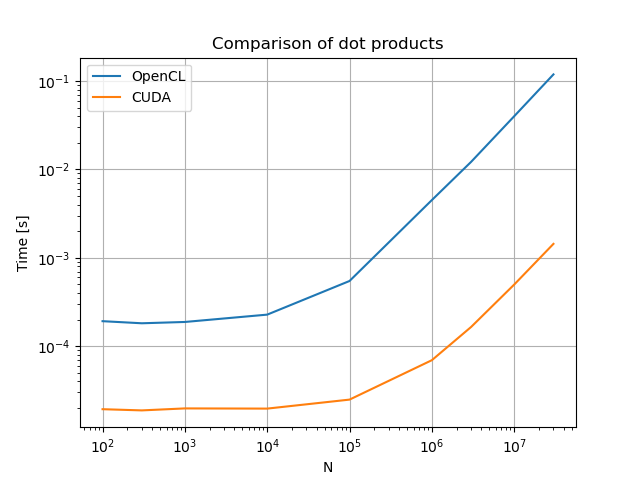
\includegraphics[scale=0.6]{plots/2.png}
\\
We can see that the CUDA version performs a lot faster. This is however not very surprising in my eyes as in that version we are using \lstinline{atomicAdd} for the summation, whereas I am using a naive summation for the OpenCL version.

\subsection{3.}
Omitted as by the newest information on the exercise page. It was not until that notice that I stopped believing that this kept failing due to my own incompetence :sweat:
\newpage
\subsection{4.}

I wrote a function that creates M kernels from ``dot0'' up to ``dot<<M-1>>'' that all perform the same steps as in task 1. I overpadded this a little so that kernel digits up to length of $4$ would be possible:

\begin{tiny}
\begin{verbatim}
const char *mSizeProgram(int M) {
  const char *init = ""
                     "#pragma OPENCL EXTENSION cl_khr_fp64 : enable\n"
                     "";
  const char *kernel_name = "__kernel void dot";
  const char *kernel_body = [...rest of dot...];
  char *var = (char *)malloc( sizeof(char) * (std::string(init).length() + M * (4 + std::string(kernel_body).length() + std::string(kernel_name).length())));
  strcpy(var, init);

  for (int i = 0; i < M; i++) {
    strcat(var, kernel_name);
    std::string no = std::to_string(i);
    char const *no_char = no.c_str();
    strcat(var, no_char);
    strcat(var, kernel_body);
  }
  const char *out = var;
  return out;
}

\end{verbatim}
\end{tiny}

The time to create these $M$ kernels was compared to the time it took to fetch one of these kernels for the given M. The results are below:\\

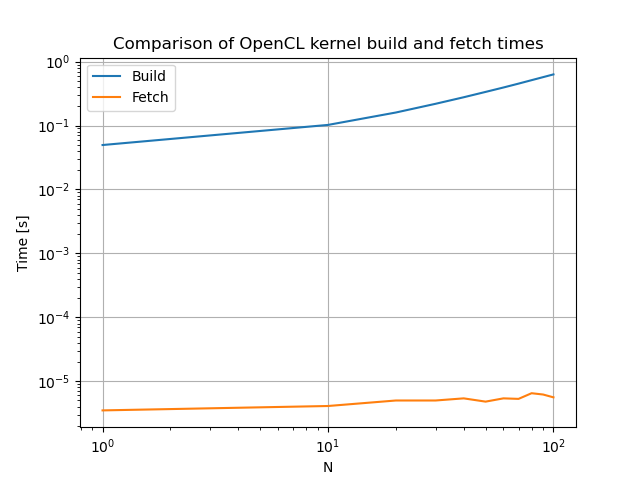
\includegraphics[scale=0.6]{plots/4.png}
\\
We can see that building is a lot slower compared to retrieval.
\newpage
\section{Implement CUDA+OpenCL (CUCL) Approach}

I implemented the following aliases for OpenCL:

\begin{verbatim}
#define STRINGIFY(ARG) #ARG
const char *my_opencl_program =
    ""
    "#define CUCL_KERNEL __kernel\n"
    "#define CUCL_GLOBALMEM __global\n"
    "#define CUCL_GLOBALID0 get_global_id(0)\n"
    "#define CUCL_GLOBALSIZE0 get_global_size(0)\n"
    "#define CUCL_LOCALMEM __local\n"
    "#define CUCL_LOCALID0 get_local_id(0)\n"
    "#define CUCL_LOCALSIZE0 get_local_size(0)\n"
    "#define CUCL_BARRIER barrier(CLK_GLOBAL_MEM_FENCE)\n"
    "#define CUCL_GROUPID0 get_group_id(0)\n"
    "#pragma OPENCL EXTENSION cl_khr_fp64 : enable\n"
#include "dot.cucl"
;
\end{verbatim}

and these for CUDA:

\begin{verbatim}
#define STRINGIFY(ARG) ARG
#define CUCL_KERNEL __global__
#define CUCL_GLOBALMEM
#define CUCL_GLOBALID0 blockDim.x *blockIdx.x + threadIdx.x
#define CUCL_GLOBALSIZE0 gridDim.x *blockDim.x
#define CUCL_LOCALMEM __shared__
#define CUCL_LOCALID0 threadIdx.x
#define CUCL_LOCALSIZE0 blockDim.x
#define CUCL_BARRIER __syncthreads()
#define CUCL_GROUPID0 blockIdx.x
#include "dot.cucl"
\end{verbatim}

\end{document}
